In this section, we will explain some concepts that are the base for our research. Before presenting microservice, we will detail the cloud computing, a distributed system that allows the utilization of microservice architecture. After introducing cloud computing, we explain the concepts about microservice, like communication patterns and the relationship with SOA (service-oriented architecture).


%Cloud computing
%%O que é?
%%Modelos de serviço
%%Middlewares de cloud
%%Características essenciais (NIST)
%%Elasticidade
%%%Definição
%%%Tipos de elasticidade
%%%Forma de tratamento da elasticidade

%Microserviços
%%Definição e engenharia de software
%%Características
%%Diferença entre microserviços e orientado a serviços

\begin{figure*}[ht]
\centering
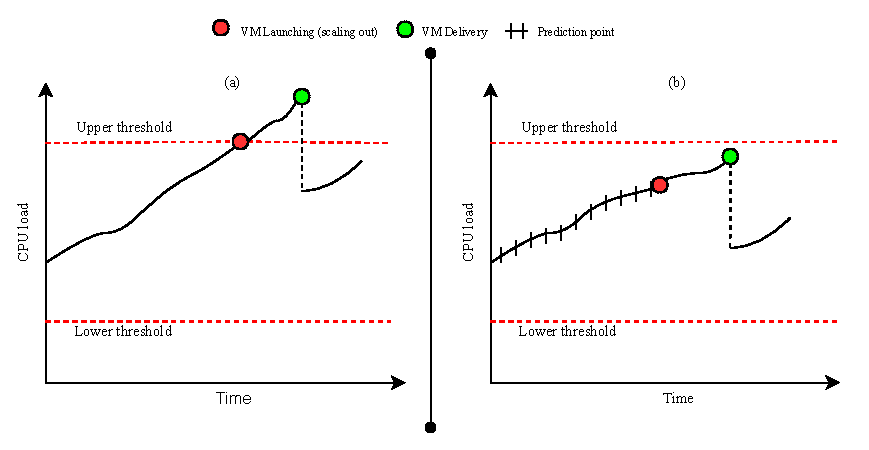
\includegraphics{Images/Previsto_real.pdf}
\caption{Elasticity approaches: (a) reactive; (b) proactive.}
\label{previsto}
\end{figure*}

%=======================================================================
% Fundamentação teórica - Cloud computing
%=======================================================================
\subsection{Cloud computing}
The network technologies improvements have proportioned reliable and high-speed access to remote resources over the Internet. These improvements have brought the idea of centralized processing to large data centers around the world, rather than running locally \cite{Marinescu2013CloudPractice}. On the other hand, this approach increased the resources sharing through the network, initially using grids and recently through Cloud computing \citep{Marinescu2013CloudPractice}.

Cloud computing is a paradigm that provides a ubiquitous network that can adjust computing resources and can quickly provisioned and released with minimal management effort or interaction with the service provider \cite{Mell2011TheComputing}. Previously, Cloud computing used as a strictly academic term. However, in recent years cloud computing appears in the most diverse services types provided over the Internet (often without the user knowing) \cite{Marinescu2013CloudPractice}.

The services models, presented by \cite{Mell2011TheComputing}, evidenced the cloud impact on early 21st-century society. Currently, \cite{Mell2011TheComputing} presents three service models:

\textbullet\ Software as a Service (SaaS): User uses an application deployed in the cloud. All the infrastructure is maintained by those who deployed the application, and the user does not manage or control the environment resources \cite{Mell2011TheComputing};

\textbullet\ Platform as a Service (PaaS): Provides an environment ready for application development. Just like in SaaS, who provides the service maintain the environment, but the user has control over the deployed applications. A PaaS example is a virtual machine configured on a server, which has the entire framework to develop Python applications \cite{Mell2011TheComputing};

\textbullet\ Infrastructure as a Service (IaaS): The cloud provider gives the infrastructure for users. Therefore, it is possible to develop or run any application, having access and control over the environment, such as network, operating system, storage, and CPU \cite{Mell2011TheComputing};

Applications like email servers (such as Gmail) are a SaaS classic example. Users do not have access to the cloud settings in which the application is running, and they only have access to the application's settings. In PaaS, we have some examples, like Pythonanywhere, service that provides a cloud environment ready for Python applications development. Finally, IaaS provides a more customizable environment, allowing network configuration, operating system definition, storage, and CPU. 

In extension to the service model, cloud computing has three deployment models, which relate to how to access these services \cite{Mell2011TheComputing}:

\textbullet\ Private cloud: Clouds provided for a specific use of an organization. Maintained by the organization, by a provider or by a mixture of the two previous ones. Typically, the cloud is in a restricted environment, without the data being available to an unregistered user;

\textbullet\ Public cloud: They are clouds managed by a provider, which provides all the infrastructure. A significant concern in this deployment model is that the provider has access to all the data storage in the cloud. On the other hand, it facilitates applications deployment without significant investments in their infrastructure;

\textbullet\ Hybrid cloud: It is a private and a public cloud combined. Hybrid is relevant in situations where an organization has a cloud (private) infrastructure but may need more resources from a public cloud.

%%Middlewares de cloud
To provide these models, several middlewares that act as the cloud manager, acting at the IaaS level. Several management tools are open source and enable Private clouds or Hybrid clouds creation. Some Open-Source middlewares examples are OpenNebula \cite{Moreno-Vozmediano2012IaaSInfrastructures}, Eucalyptus \cite{Nurmi2009TheSystem}, and OpenStack \cite{Sefraoui2012OpenStack:Computing}. An essential public clouds feature is the pay-as-you-go concept, which consists of charging the user for the usage time and the amount of resources allocation.

Any cloud management middleware provides an application programming interface (API), additionally to a graphical or command line interface. With this API, anyone can develop applications that monitor and manage features according to users needs and application behavior. Several academic examples use the API to develop solutions, such as \cite{DaRosaRighi2016Autoelastic:Cloud}, \cite{Molto2013ElasticRequirements}, \cite{Spinner2014RuntimeEstimation}, \cite{Beernaert2012AutomaticOpenStack}, \cite{Roy2011EfficientForecasting}, \cite{Loff2014Vadara:Applications}, and \cite{Rosa2014AnMechanisms}.

Cloud computing is only possible due to resources virtualization through virtual machines (VMs). VMs can perform the same computational functions that a physical computer \cite{Birman2012GuideSystems}. Typically, exists data centers that allow allocating multiple virtual machines according to the user needs \cite{Marinescu2013CloudPractice}. This virtualization provides some benefits over the predecessor multicomputers, like clusters and grids. The first one is simplified management, requiring few managers to set up and release new features \cite{Birman2012GuideSystems}. Through access interfaces (graphical, command line or programming), it is possible to adjust virtual machine configurations, such as memory, CPU, and others. In comparison to physical media, changing some of these settings requires buying hardware and spending hours installing and configuring \cite{Birman2012GuideSystems}.

Another strong point of cloud computing is green computing. With the right Cloud computing management it is possible to keep active only the needed VMs \cite{Righi2013ElasticidadeDesafios}. Besides, cloud servers are optimized. They use less energy cost compared to physical machines with similar resources.

Until then, anything is different from something already presented in another distributed systems. The high differential of the cloud computing model is the elasticity \cite{Righi2013ElasticidadeDesafios}.

%%Elasticidade
\begin{figure*}[ht]
\centering
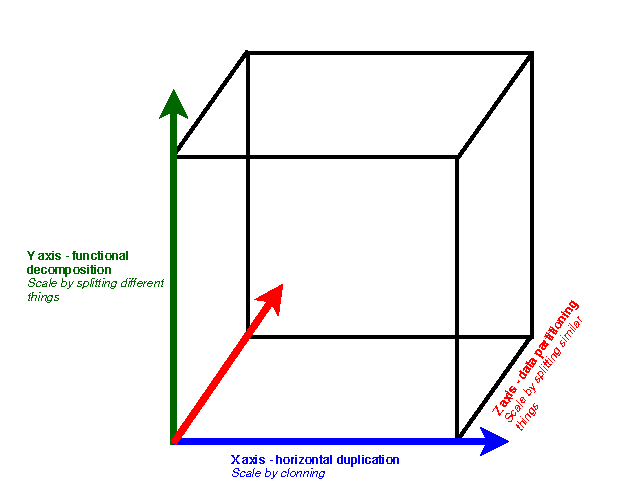
\includegraphics{Images/ScaleCube.pdf}
\caption{Scale cube \cite{MartinL.Abbott2015TheLivros}}
\label{scaleCube}
\end{figure*}


\subsection{Elasticity}

%%%Definição
Elasticity is one of the most significant cloud computing features \cite{Molto2013ElasticRequirements}. Elasticity is the ability to adapt the resources on the fly according to need. There are two types of elasticity in cloud computing \cite{Righi2013ElasticidadeDesafios}. 

%%%Tipos de elasticidade
The first one is horizontal elasticity, which quickly provisions and releases computational nodes (virtual machines)  \cite{Molto2013ElasticRequirements}. This elasticity is frequently used to adjust cloud according to changes in workload and to avoid additional costs. For example, there is a virtual machine in charge of dealing with web requests. At a specific time of the day, the number of request increase and only one machine is not enough. Thus, by identifying this peak, the manager can (manually or automatically) instantiate new machines quickly.

The other elasticity form is vertical, which is the ability to adjust virtual machines settings, increasing or decreasing their capacity \cite{Spinner2014RuntimeEstimation}. In other words, vertical elasticity is the possibility to increase resources, such as CPU, memory, and network type, without the need for hardware changes. The weakness in this approach is that some middlewares, such as OpenNebula, require to turn off the virtual machine to adjust some of its parameters (such as CPU) \cite{Moreno-Vozmediano2012IaaSInfrastructures}.

Regardless of the elasticity type, this is a crucial element to improve application performance. For example, it is possible to add new virtual machines to perform tasks (horizontal elasticity) or increase some virtual machine resource (vertical elasticity) so that it can finish its task faster \cite{Righi2013ElasticidadeDesafios}. 

%%%Forma de tratamento da elasticidade
Resources allocation can follow two approaches \cite{Righi2013ElasticidadeDesafios}. The first one is the manual resources allocation, which requires user action. Public and private middlewares have tools to make these adjustments, usually through a graphical interface, command line or programming API \cite{Righi2013ElasticidadeDesafios}. The second approach is automatic and has two types of treatment: reactive and proactive \cite{Righi2013ElasticidadeDesafios}. 

In the reactive form, according to statically defined rules is to perform elasticity decisions. Commercial systems, such as Amazon AWS, Nimbus, and Windows Azure, use this way to provide elasticity \cite{Righi2013ElasticidadeDesafios}. The rules define metrics thresholds and the elasticity action to perform when thresholds reach. A cloud receives these rules through a Service Level Objective (SLO) \cite{Spinner2014RuntimeEstimation}. A reactive elasticity example is to indicate that if a virtual machine reaches 20\% CPU, it needs turning off (horizontal elasticity) or it must decrease its total CPU (vertical elasticity).

The cloud adapts according to the thresholds defined in SLO. However, reactive elasticity has two significant problems. The first one is how to define the best thresholds for a given application. This definition is not trivial and requires ability from user to configure management tool besides an analysis of each application separately \cite{Righi2013ElasticidadeDesafios}.

The second problem is that the reactive elasticity performs an action when a resource reaches an undesirable state (defined by the threshold). In horizontal elasticity, after triggering the adding a new resource action, there is an interval to starts this resource. Then, after reaching an undesirable state, it will remain in that state until the new feature is ready. This time varies for each cloud manager, VM size,  and host hardware, but some authors indicate that the virtual machine instantiation time is between 5 and 15 minutes \cite{Bankole2013CloudEnvironment, Brebner2012IsEnough}.

The proactive approach aims to solve the reactive problems (mainly, the second one). This approach used historical data to detect patterns and to predict the best time to act \cite{Righi2013ElasticidadeDesafios}. Thus, the forecast uses the resource initialization time and this smooth the violation problem. Machine learning or time series calculations are the algorithms usually used for this prediction \cite{Rosa2014AnMechanisms, Gong2010PRESS:Systems, Loff2014Vadara:Applications, Roy2011EfficientForecasting, Moore2013TransformingAuto-scaling, Barrett2013ApplyingCloud, Nikravesh2017AnProvisioning}. Figure~\ref{previsto} demonstrates the reactive and proactive behaviors. In (a) exemplifies how the CPU of a system could behave in the reactive form. A VM launch when CPU reaches a threshold. The CPU stays in an undesirable state until the VM is ready. In (b) exemplifies the proactive approach. The system predicts that will be necessary to instantiate a new virtual machine. Then, the manager instantiates a new resource to deal with CPU peak. When the virtual machine is ready generates a CPU smoothing. 

\begin{figure*}[th]
\centering
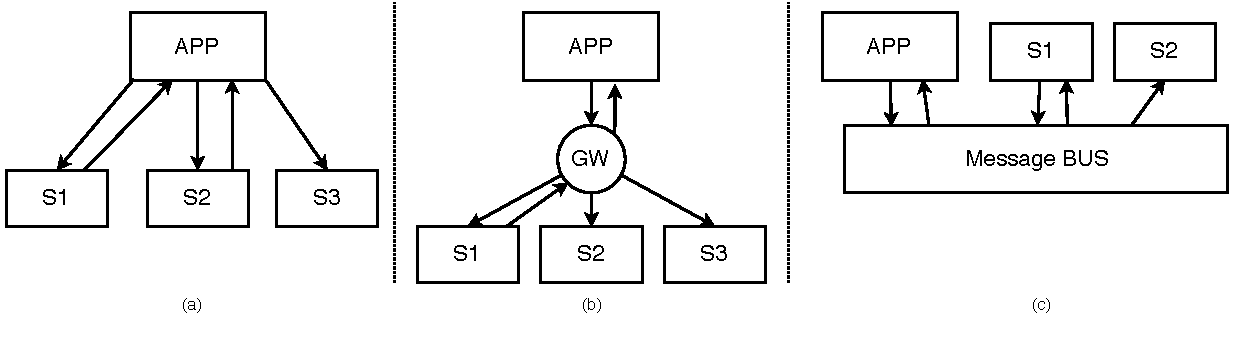
\includegraphics[scale=0.8]{Images/Microservices_comm.pdf}
\caption{Patterns of communication through microservices \cite{Namiot2014OnArchitecture}. (a) The application communicates directly with the services. (b) The gateway receives the requisition and passes it to the appropriate microservice. (c) Message bus where the application and services communicate through it.}
\label{microcomm}
\end{figure*}

As mentioned earlier, a web server is an example of the use of elasticity, which, according to the workload, adds more VMs to handle the requests increase. This approach is a classic example of elasticity that uses the replication strategy \cite{Righi2013ElasticidadeDesafios}. In this strategy, there is a pre-configured virtual machine template of application. This template is used to create a new virtual machine when necessary. Typically, the replicated machines do not communicate with each other, but through a centralizer that distributes tasks \cite{Righi2013ElasticidadeDesafios}. Also, these machines can exchange information through shared memory. In addition to web applications, high-performance applications, such as those following the master-slave model, can use the replication approach \cite{Righi2013ElasticidadeDesafios}.

Besides the above strategy, two others can be used to provide elasticity \cite{Righi2013ElasticidadeDesafios}. The first is resource migration, which consists of migrating VMs between physical resources. Regarding performance, several middlewares allow this migration in acceptable terms, and this strategy is particularly interesting concerning energy consumption \cite{Righi2013ElasticidadeDesafios}. It is possible to join virtual machines of different physical resources, allowing resources disconnection.

Finally, the last is the resizing strategy. An example of this strategy is to adjust the percentage of CPU used by a virtual machine so that it finishes its processing faster. Resizing is not exclusive to CPU, for example, this could also adjust the bandwidth of a virtual private network \cite{Righi2013ElasticidadeDesafios}. Not all cloud computing middlewares enable on-the-fly scaling, requiring virtual machine shutdown before resizing. Regarding high-performance applications, this is particularly critical as it would require a time-out, resizing, and initialization.

Elasticity can improve the performance of a large variety of applications type submitted to the cloud. However, an architecture approach is growing its utilization combined with a cloud. This approach is microservice.

%=======================================================================
% Fundamentação teórica - Microserviços
%=======================================================================
\subsection{Microservices}

%Intro
The most traditional architecture to develop an application, independent of the application purpose, is monolithic. In small applications, this architecture has several advantages, such as simplicity of development, testing and deploying \cite{Chen2017FromApproach}. However, as applications increase and grow complexity, these advantages tend to become disadvantages. For example, implement new features without inserting bugs becomes more complicated, since the developer does not know all the impact of their changes. 

Another limitation of large monolithic applications is scalability \cite{Chen2017FromApproach}. For example, to handle an increase in requests a cloud needs invoke more instances of the application. In monolithic, the entire application needs to replicate. However, perhaps only a part of the applications needs to replicate.

%%Motivação
To mitigate these disadvantages, an approach that is increasing followers, both academia and industry, is the architecture based on microservices ~\cite{Chen2017FromApproach}. Microservices consists of developing an application creating several small and independent services \cite{Namiot2014OnArchitecture}. 

This development approach has grown in recent years but is not something new. The term microservices has emerged in the agile development community since 2014 \cite{Zimmermann2017MicroservicesDeployment}. Some authors consider Microservices as a new approach to the Service-Oriented Architecture (SOA) architecture, which primarily consists of dividing an application into services ~\cite{Zimmermann2017MicroservicesDeployment}. However, there is no agreement on the relationship between microservices and SOA \cite{Chen2017FromApproach}.

%Definição e engenharia de software
This architecture consists of a set of small services with the least possible responsibility. In other words, a service has a well-defined function in the system. These services communicated through a lightweight protocol (such as HTTP) \cite{Namiot2014OnArchitecture}. So, unlike the monolithic approach which has an application only, in microservices we have several separate services that can communicate with each other. These services do not have to be written in the same programming language, allowing implement the best strategy for each new service.

%%Comparação com monolítico
Thus, an architecture based on microservices becomes attractive in comparison to monolithic architectures for several reasons. Developing new features becomes simple since the scope of the service is well-defined with little coupling between services. In monolithic applications, there is usually a high coupling between classes \cite{Namiot2014OnArchitecture}. 

Another consideration for the comparison between these two architectures is the scalability. The scale cube, shown in figure~\ref{scaleCube}, describes the approaches to provide scalability to an application \cite{Namiot2014OnArchitecture}. At the start point, there is a monolithic application with no scalability. A monolithic application can scale by adding new replicas of the application, represented in figure~\ref{scaleCube} as the X-axis.

Another way to provide scalability can be by splitting the data of an application. In this way, each server runs an identical application, but each one is responsible for a part of the data \cite{Namiot2014OnArchitecture}. An example of this is database sharding, which consists in using the primary key of a table to data routing \cite{Namiot2014OnArchitecture}. The z-axis in figure~\ref{scaleCube} exemplifies this scalability

Adding new replicas or splitting the data can increase the scalability of the monolithic application without performing a decomposition of services, but this can increase the complexity of the system \cite{Namiot2014OnArchitecture}. While data decomposition split similar things, decomposing functions divide a large system into smaller (micro) services that do different things \cite{Namiot2014OnArchitecture}. Thus, a monolithic application becomes a set of small services, and the scaler manager can replicate these services individually.

These concepts can be applied in combination, aiming at a better performance of the application. For example, the developer can divide a large application into several microservices, applying functional decomposition. While in a monolithic system a requisition executes the entire application, with the decomposition, the requisition performs just the required service.  This division could be enough to increase the performance and scalability of the system, but If it is not enough, the developer can combine the replication of a critical service.

While in monolithic systems communication is not critical, in microservices, just like any distributed system, it becomes a crucial point. Services are in constant communication with each other and with external applications. The figure~\ref{microcomm} shows three communication patterns \cite{Namiot2014OnArchitecture}. 

In (a) we have an application communicating directly with the services, without any intermediary. This approach offers a simple implementation and management. However, when it is necessary to apply the replication of some services, it will be necessary to modify the application and services. This modification becomes necessary because there is no load balancer to route the application request to the correct service. Also, both the application and the services must use the same communication protocol. The communication protocol can be a significant problem because the services are heterogeneous, requiring the application to implement all the communication protocols of the services it wants to communicate. Usually, services implement the HTTP protocol.

Thus, the pattern (b) of figure~\ref{microcomm} that, unlike the previous model, adds a gateway between applications and services \cite{Namiot2014OnArchitecture}. The gateway knows the protocol of all the services of its system, giving to the applications a unique communication protocol. Besides, the gateway rotates the requests for services. With this routing, the system can add new nodes without changing applications and services.

Another pattern of communication is presented in (c), where there is a single communication bus used by both applications and services. Like the previous model, this model also enables the replication of services, but the services need to verify which requests are their responsibility. Also, there must be a way to indicate that a service is processing a request, so that two microservices do not process the same thing.